\documentclass[1p]{elsarticle_modified}
%\bibliographystyle{elsarticle-num}

%\usepackage[colorlinks]{hyperref}
%\usepackage{abbrmath_seonhwa} %\Abb, \Ascr, \Acal ,\Abf, \Afrak
\usepackage{amsfonts}
\usepackage{amssymb}
\usepackage{amsmath}
\usepackage{amsthm}
\usepackage{scalefnt}
\usepackage{amsbsy}
\usepackage{kotex}
\usepackage{caption}
\usepackage{subfig}
\usepackage{color}
\usepackage{graphicx}
\usepackage{xcolor} %% white, black, red, green, blue, cyan, magenta, yellow
\usepackage{float}
\usepackage{setspace}
\usepackage{hyperref}

\usepackage{tikz}
\usetikzlibrary{arrows}

\usepackage{multirow}
\usepackage{array} % fixed length table
\usepackage{hhline}

%%%%%%%%%%%%%%%%%%%%%
\makeatletter
\renewcommand*\env@matrix[1][\arraystretch]{%
	\edef\arraystretch{#1}%
	\hskip -\arraycolsep
	\let\@ifnextchar\new@ifnextchar
	\array{*\c@MaxMatrixCols c}}
\makeatother %https://tex.stackexchange.com/questions/14071/how-can-i-increase-the-line-spacing-in-a-matrix
%%%%%%%%%%%%%%%

\usepackage[normalem]{ulem}

\newcommand{\msout}[1]{\ifmmode\text{\sout{\ensuremath{#1}}}\else\sout{#1}\fi}
%SOURCE: \msout is \stkout macro in https://tex.stackexchange.com/questions/20609/strikeout-in-math-mode

\newcommand{\cancel}[1]{
	\ifmmode
	{\color{red}\msout{#1}}
	\else
	{\color{red}\sout{#1}}
	\fi
}

\newcommand{\add}[1]{
	{\color{blue}\uwave{#1}}
}

\newcommand{\replace}[2]{
	\ifmmode
	{\color{red}\msout{#1}}{\color{blue}\uwave{#2}}
	\else
	{\color{red}\sout{#1}}{\color{blue}\uwave{#2}}
	\fi
}

\newcommand{\Sol}{\mathcal{S}} %segment
\newcommand{\D}{D} %diagram
\newcommand{\A}{\mathcal{A}} %arc


%%%%%%%%%%%%%%%%%%%%%%%%%%%%%5 test

\def\sl{\operatorname{\textup{SL}}(2,\Cbb)}
\def\psl{\operatorname{\textup{PSL}}(2,\Cbb)}
\def\quan{\mkern 1mu \triangleright \mkern 1mu}

\theoremstyle{definition}
\newtheorem{thm}{Theorem}[section]
\newtheorem{prop}[thm]{Proposition}
\newtheorem{lem}[thm]{Lemma}
\newtheorem{ques}[thm]{Question}
\newtheorem{cor}[thm]{Corollary}
\newtheorem{defn}[thm]{Definition}
\newtheorem{exam}[thm]{Example}
\newtheorem{rmk}[thm]{Remark}
\newtheorem{alg}[thm]{Algorithm}

\newcommand{\I}{\sqrt{-1}}
\begin{document}

%\begin{frontmatter}
%
%\title{Boundary parabolic representations of knots up to 8 crossings}
%
%%% Group authors per affiliation:
%\author{Yunhi Cho} 
%\address{Department of Mathematics, University of Seoul, Seoul, Korea}
%\ead{yhcho@uos.ac.kr}
%
%
%\author{Seonhwa Kim} %\fnref{s_kim}}
%\address{Center for Geometry and Physics, Institute for Basic Science, Pohang, 37673, Korea}
%\ead{ryeona17@ibs.re.kr}
%
%\author{Hyuk Kim}
%\address{Department of Mathematical Sciences, Seoul National University, Seoul 08826, Korea}
%\ead{hyukkim@snu.ac.kr}
%
%\author{Seokbeom Yoon}
%\address{Department of Mathematical Sciences, Seoul National University, Seoul, 08826,  Korea}
%\ead{sbyoon15@snu.ac.kr}
%
%\begin{abstract}
%We find all boundary parabolic representation of knots up to 8 crossings.
%
%\end{abstract}
%\begin{keyword}
%    \MSC[2010] 57M25 
%\end{keyword}
%
%\end{frontmatter}

%\linenumbers
%\tableofcontents
%
\newcommand\colored[1]{\textcolor{white}{\rule[-0.35ex]{0.8em}{1.4ex}}\kern-0.8em\color{red} #1}%
%\newcommand\colored[1]{\textcolor{white}{ #1}\kern-2.17ex	\textcolor{white}{ #1}\kern-1.81ex	\textcolor{white}{ #1}\kern-2.15ex\color{red}#1	}

{\Large $\underline{12a_{1118}~(K12a_{1118})}$}

\setlength{\tabcolsep}{10pt}
\renewcommand{\arraystretch}{1.6}
\vspace{1cm}\begin{tabular}{m{100pt}>{\centering\arraybackslash}m{274pt}}
\multirow{5}{120pt}{
	\centering
	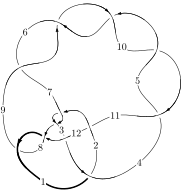
\includegraphics[width=112pt]{../../../GIT/diagram.site/Diagrams/png/1919_12a_1118.png}\\
\ \ \ A knot diagram\footnotemark}&
\allowdisplaybreaks
\textbf{Linearized knot diagam} \\
\cline{2-2}
 &
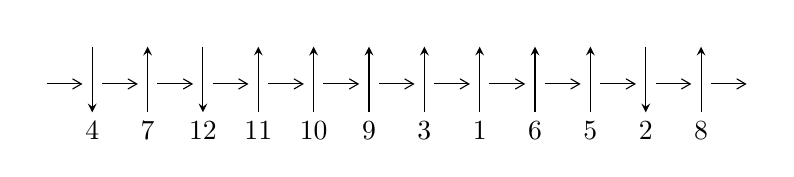
\begin{tikzpicture}[x=20pt, y=17pt]
	% nodes
	\node (C0) at (0, 0) {};
	\node (C1) at (1, 0) {};
	\node (C1U) at (1, +1) {};
	\node (C1D) at (1, -1) {4};

	\node (C2) at (2, 0) {};
	\node (C2U) at (2, +1) {};
	\node (C2D) at (2, -1) {7};

	\node (C3) at (3, 0) {};
	\node (C3U) at (3, +1) {};
	\node (C3D) at (3, -1) {12};

	\node (C4) at (4, 0) {};
	\node (C4U) at (4, +1) {};
	\node (C4D) at (4, -1) {11};

	\node (C5) at (5, 0) {};
	\node (C5U) at (5, +1) {};
	\node (C5D) at (5, -1) {10};

	\node (C6) at (6, 0) {};
	\node (C6U) at (6, +1) {};
	\node (C6D) at (6, -1) {9};

	\node (C7) at (7, 0) {};
	\node (C7U) at (7, +1) {};
	\node (C7D) at (7, -1) {3};

	\node (C8) at (8, 0) {};
	\node (C8U) at (8, +1) {};
	\node (C8D) at (8, -1) {1};

	\node (C9) at (9, 0) {};
	\node (C9U) at (9, +1) {};
	\node (C9D) at (9, -1) {6};

	\node (C10) at (10, 0) {};
	\node (C10U) at (10, +1) {};
	\node (C10D) at (10, -1) {5};

	\node (C11) at (11, 0) {};
	\node (C11U) at (11, +1) {};
	\node (C11D) at (11, -1) {2};

	\node (C12) at (12, 0) {};
	\node (C12U) at (12, +1) {};
	\node (C12D) at (12, -1) {8};
	\node (C13) at (13, 0) {};

	% arrows
	\draw[->,>={angle 60}]
	(C0) edge (C1) (C1) edge (C2) (C2) edge (C3) (C3) edge (C4) (C4) edge (C5) (C5) edge (C6) (C6) edge (C7) (C7) edge (C8) (C8) edge (C9) (C9) edge (C10) (C10) edge (C11) (C11) edge (C12) (C12) edge (C13) ;	\draw[->,>=stealth]
	(C1U) edge (C1D) (C2D) edge (C2U) (C3U) edge (C3D) (C4D) edge (C4U) (C5D) edge (C5U) (C6D) edge (C6U) (C7D) edge (C7U) (C8D) edge (C8U) (C9D) edge (C9U) (C10D) edge (C10U) (C11U) edge (C11D) (C12D) edge (C12U) ;
	\end{tikzpicture} \\
\hhline{~~} \\& 
\textbf{Solving Sequence} \\ \cline{2-2} 
 &
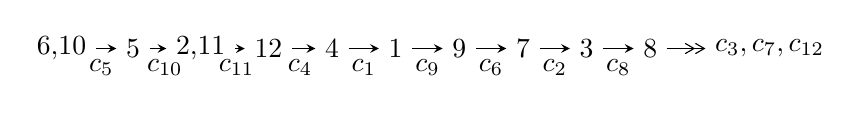
\begin{tikzpicture}[x=23pt, y=7pt]
	% node
	\node (A0) at (-1/8, 0) {6,10};
	\node (A1) at (1, 0) {5};
	\node (A2) at (33/16, 0) {2,11};
	\node (A3) at (25/8, 0) {12};
	\node (A4) at (33/8, 0) {4};
	\node (A5) at (41/8, 0) {1};
	\node (A6) at (49/8, 0) {9};
	\node (A7) at (57/8, 0) {7};
	\node (A8) at (65/8, 0) {3};
	\node (A9) at (73/8, 0) {8};
	\node (C1) at (1/2, -1) {$c_{5}$};
	\node (C2) at (3/2, -1) {$c_{10}$};
	\node (C3) at (21/8, -1) {$c_{11}$};
	\node (C4) at (29/8, -1) {$c_{4}$};
	\node (C5) at (37/8, -1) {$c_{1}$};
	\node (C6) at (45/8, -1) {$c_{9}$};
	\node (C7) at (53/8, -1) {$c_{6}$};
	\node (C8) at (61/8, -1) {$c_{2}$};
	\node (C9) at (69/8, -1) {$c_{8}$};
	\node (A10) at (11, 0) {$c_{3},c_{7},c_{12}$};

	% edge
	\draw[->,>=stealth]	
	(A0) edge (A1) (A1) edge (A2) (A2) edge (A3) (A3) edge (A4) (A4) edge (A5) (A5) edge (A6) (A6) edge (A7) (A7) edge (A8) (A8) edge (A9) ;
	\draw[->>,>={angle 60}]	
	(A9) edge (A10);
\end{tikzpicture} \\ 

\end{tabular} \\

\footnotetext{
The image of knot diagram is generated by the software ``\textbf{Draw programme}" developed by Andrew Bartholomew(\url{http://www.layer8.co.uk/maths/draw/index.htm\#Running-draw}), where we modified some parts for our purpose(\url{https://github.com/CATsTAILs/LinksPainter}).
}\phantom \\ \newline 
\centering \textbf{Ideals for irreducible components\footnotemark of $X_{\text{par}}$} 
 
\begin{align*}
I^u_{1}&=\langle 
- u^{25}+6 u^{24}+\cdots+2 b+2,\;u^{25}-4 u^{24}+\cdots+4 a-28,\;u^{26}-6 u^{25}+\cdots+38 u-4\rangle \\
I^u_{2}&=\langle 
23119780 u^{10} a^3-26302390 u^{10} a^2+\cdots-9354998 a+21323123,\;u^{10} a^2-2 u^{10} a+\cdots-4 a+22,\\
\phantom{I^u_{2}}&\phantom{= \langle  }u^{11}+u^{10}+8 u^9+7 u^8+22 u^7+16 u^6+24 u^5+13 u^4+9 u^3+3 u^2-1\rangle \\
I^u_{3}&=\langle 
u^{11}+2 u^{10}+9 u^9+14 u^8+29 u^7+34 u^6+40 u^5+33 u^4+21 u^3+10 u^2+b+2 u,\\
\phantom{I^u_{3}}&\phantom{= \langle  }u^9+2 u^8+8 u^7+12 u^6+22 u^5+23 u^4+24 u^3+15 u^2+a+8 u+2,\\
\phantom{I^u_{3}}&\phantom{= \langle  }u^{13}+u^{12}+10 u^{11}+9 u^{10}+38 u^9+30 u^8+68 u^7+45 u^6+57 u^5+30 u^4+18 u^3+9 u^2+1\rangle \\
\\
\end{align*}
\raggedright * 3 irreducible components of $\dim_{\mathbb{C}}=0$, with total 83 representations.\\
\footnotetext{All coefficients of polynomials are rational numbers. But the coefficients are sometimes approximated in decimal forms when there is not enough margin.}
\newpage
\renewcommand{\arraystretch}{1}
\centering \section*{I. $I^u_{1}= \langle - u^{25}+6 u^{24}+\cdots+2 b+2,\;u^{25}-4 u^{24}+\cdots+4 a-28,\;u^{26}-6 u^{25}+\cdots+38 u-4 \rangle$}
\flushleft \textbf{(i) Arc colorings}\\
\begin{tabular}{m{7pt} m{180pt} m{7pt} m{180pt} }
\flushright $a_{6}=$&$\begin{pmatrix}1\\0\end{pmatrix}$ \\
\flushright $a_{10}=$&$\begin{pmatrix}0\\u\end{pmatrix}$ \\
\flushright $a_{5}=$&$\begin{pmatrix}1\\u^2\end{pmatrix}$ \\
\flushright $a_{2}=$&$\begin{pmatrix}-\frac{1}{4} u^{25}+u^{24}+\cdots-\frac{141}{4} u+7\\\frac{1}{2} u^{25}-3 u^{24}+\cdots-\frac{1}{2} u-1\end{pmatrix}$ \\
\flushright $a_{11}=$&$\begin{pmatrix}u\\u^3+u\end{pmatrix}$ \\
\flushright $a_{12}=$&$\begin{pmatrix}- u^{25}+\frac{11}{2} u^{24}+\cdots+73 u-\frac{21}{2}\\\frac{1}{2} u^{25}-3 u^{24}+\cdots-\frac{27}{2} u+2\end{pmatrix}$ \\
\flushright $a_{4}=$&$\begin{pmatrix}u^2+1\\u^4+2 u^2\end{pmatrix}$ \\
\flushright $a_{1}=$&$\begin{pmatrix}\frac{1}{4} u^{25}-2 u^{24}+\cdots-\frac{271}{4} u+10\\\frac{1}{2} u^{25}-2 u^{24}+\cdots+\frac{7}{2} u-1\end{pmatrix}$ \\
\flushright $a_{9}=$&$\begin{pmatrix}- u\\u\end{pmatrix}$ \\
\flushright $a_{7}=$&$\begin{pmatrix}u^2+1\\- u^2\end{pmatrix}$ \\
\flushright $a_{3}=$&$\begin{pmatrix}\frac{1}{4} u^{25}- u^{24}+\cdots-\frac{71}{4} u+4\\-\frac{1}{2} u^{25}+2 u^{24}+\cdots+\frac{3}{2} u-1\end{pmatrix}$ \\
\flushright $a_{8}=$&$\begin{pmatrix}- u^{25}+\frac{11}{2} u^{24}+\cdots+42 u-\frac{9}{2}\\-\frac{1}{2} u^{25}+3 u^{24}+\cdots+\frac{71}{2} u-4\end{pmatrix}$\\&\end{tabular}
\flushleft \textbf{(ii) Obstruction class $= -1$}\\~\\
\flushleft \textbf{(iii) Cusp Shapes $= 10 u^{25}-57 u^{24}+332 u^{23}-1235 u^{22}+4198 u^{21}-11498 u^{20}+28340 u^{19}-60404 u^{18}+115879 u^{17}-197385 u^{16}+302899 u^{15}-416264 u^{14}+513994 u^{13}-567135 u^{12}+556938 u^{11}-481994 u^{10}+362452 u^9-230985 u^8+118944 u^7-43997 u^6+6370 u^5+5367 u^4-5117 u^3+2313 u^2-586 u+70$}\\~\\
\newpage\renewcommand{\arraystretch}{1}
\flushleft \textbf{(iv) u-Polynomials at the component}\newline \\
\begin{tabular}{m{50pt}|m{274pt}}
Crossings & \hspace{64pt}u-Polynomials at each crossing \\
\hline $$\begin{aligned}c_{1},c_{11}\end{aligned}$$&$\begin{aligned}
&u^{26}-8 u^{24}+\cdots+12 u-1
\end{aligned}$\\
\hline $$\begin{aligned}c_{2},c_{7},c_{8}\\c_{12}\end{aligned}$$&$\begin{aligned}
&u^{26}+u^{25}+\cdots-2 u^2+1
\end{aligned}$\\
\hline $$\begin{aligned}c_{3}\end{aligned}$$&$\begin{aligned}
&u^{26}+22 u^{25}+\cdots-18432 u-2048
\end{aligned}$\\
\hline $$\begin{aligned}c_{4},c_{5},c_{6}\\c_{9},c_{10}\end{aligned}$$&$\begin{aligned}
&u^{26}+6 u^{25}+\cdots-38 u-4
\end{aligned}$\\
\hline
\end{tabular}\\~\\
\newpage\renewcommand{\arraystretch}{1}
\flushleft \textbf{(v) Riley Polynomials at the component}\newline \\
\begin{tabular}{m{50pt}|m{274pt}}
Crossings & \hspace{64pt}Riley Polynomials at each crossing \\
\hline $$\begin{aligned}c_{1},c_{11}\end{aligned}$$&$\begin{aligned}
&y^{26}-16 y^{25}+\cdots-70 y+1
\end{aligned}$\\
\hline $$\begin{aligned}c_{2},c_{7},c_{8}\\c_{12}\end{aligned}$$&$\begin{aligned}
&y^{26}-17 y^{25}+\cdots-4 y+1
\end{aligned}$\\
\hline $$\begin{aligned}c_{3}\end{aligned}$$&$\begin{aligned}
&y^{26}+4 y^{25}+\cdots-27262976 y+4194304
\end{aligned}$\\
\hline $$\begin{aligned}c_{4},c_{5},c_{6}\\c_{9},c_{10}\end{aligned}$$&$\begin{aligned}
&y^{26}+34 y^{25}+\cdots-44 y+16
\end{aligned}$\\
\hline
\end{tabular}\\~\\
\newpage\flushleft \textbf{(vi) Complex Volumes and Cusp Shapes}
$$\begin{array}{c|c|c}  
\text{Solutions to }I^u_{1}& \I (\text{vol} + \sqrt{-1}CS) & \text{Cusp shape}\\
 \hline 
\begin{aligned}
u &= \phantom{-}0.451485 + 0.924968 I \\
a &= -0.130539 + 0.087112 I \\
b &= -0.420502 + 1.028160 I\end{aligned}
 & -1.83398 + 3.85554 I & \phantom{-}5.01598 - 5.40942 I \\ \hline\begin{aligned}
u &= \phantom{-}0.451485 - 0.924968 I \\
a &= -0.130539 - 0.087112 I \\
b &= -0.420502 - 1.028160 I\end{aligned}
 & -1.83398 - 3.85554 I & \phantom{-}5.01598 + 5.40942 I \\ \hline\begin{aligned}
u &= \phantom{-}0.145760 + 1.021400 I \\
a &= -0.753104 + 0.547406 I \\
b &= \phantom{-}0.342480 + 0.917771 I\end{aligned}
 & -5.29967 + 2.25279 I & -2.26265 - 1.02341 I \\ \hline\begin{aligned}
u &= \phantom{-}0.145760 - 1.021400 I \\
a &= -0.753104 - 0.547406 I \\
b &= \phantom{-}0.342480 - 0.917771 I\end{aligned}
 & -5.29967 - 2.25279 I & -2.26265 + 1.02341 I \\ \hline\begin{aligned}
u &= -0.134335 + 1.100410 I \\
a &= \phantom{-}0.416493 - 0.318786 I \\
b &= -0.390034 - 0.369021 I\end{aligned}
 & -2.74898 - 2.01553 I & \phantom{-}1.43698 + 3.09740 I \\ \hline\begin{aligned}
u &= -0.134335 - 1.100410 I \\
a &= \phantom{-}0.416493 + 0.318786 I \\
b &= -0.390034 + 0.369021 I\end{aligned}
 & -2.74898 + 2.01553 I & \phantom{-}1.43698 - 3.09740 I \\ \hline\begin{aligned}
u &= \phantom{-}0.396788 + 1.050250 I \\
a &= \phantom{-}0.134501 - 0.556460 I \\
b &= \phantom{-}0.016917 - 1.255860 I\end{aligned}
 & \phantom{-}1.46402 + 12.63110 I & \phantom{-}4.83525 - 8.43212 I \\ \hline\begin{aligned}
u &= \phantom{-}0.396788 - 1.050250 I \\
a &= \phantom{-}0.134501 + 0.556460 I \\
b &= \phantom{-}0.016917 + 1.255860 I\end{aligned}
 & \phantom{-}1.46402 - 12.63110 I & \phantom{-}4.83525 + 8.43212 I \\ \hline\begin{aligned}
u &= \phantom{-}0.600772 + 0.564810 I \\
a &= -0.561165 - 0.113187 I \\
b &= \phantom{-}0.746852 - 0.565960 I\end{aligned}
 & \phantom{-}4.56542 - 4.85080 I & \phantom{-}7.22981 + 3.61746 I \\ \hline\begin{aligned}
u &= \phantom{-}0.600772 - 0.564810 I \\
a &= -0.561165 + 0.113187 I \\
b &= \phantom{-}0.746852 + 0.565960 I\end{aligned}
 & \phantom{-}4.56542 + 4.85080 I & \phantom{-}7.22981 - 3.61746 I\\
 \hline 
 \end{array}$$\newpage$$\begin{array}{c|c|c}  
\text{Solutions to }I^u_{1}& \I (\text{vol} + \sqrt{-1}CS) & \text{Cusp shape}\\
 \hline 
\begin{aligned}
u &= \phantom{-}0.670718 + 0.249321 I \\
a &= -0.759309 + 1.103710 I \\
b &= -0.558746 - 0.364300 I\end{aligned}
 & \phantom{-}5.48801 + 9.02308 I & \phantom{-}9.08097 - 7.68820 I \\ \hline\begin{aligned}
u &= \phantom{-}0.670718 - 0.249321 I \\
a &= -0.759309 - 1.103710 I \\
b &= -0.558746 + 0.364300 I\end{aligned}
 & \phantom{-}5.48801 - 9.02308 I & \phantom{-}9.08097 + 7.68820 I \\ \hline\begin{aligned}
u &= \phantom{-}0.690457\phantom{ +0.000000I} \\
a &= \phantom{-}1.22468\phantom{ +0.000000I} \\
b &= \phantom{-}0.250949\phantom{ +0.000000I}\end{aligned}
 & \phantom{-}0.998593\phantom{ +0.000000I} & \phantom{-}8.67860\phantom{ +0.000000I} \\ \hline\begin{aligned}
u &= \phantom{-}0.20001 + 1.43415 I \\
a &= \phantom{-}0.643331 - 0.201919 I \\
b &= -0.264059 + 0.214501 I\end{aligned}
 & -1.89647 - 1.89309 I & \phantom{-0.000000 -}0. + 6.08456 I \\ \hline\begin{aligned}
u &= \phantom{-}0.20001 - 1.43415 I \\
a &= \phantom{-}0.643331 + 0.201919 I \\
b &= -0.264059 - 0.214501 I\end{aligned}
 & -1.89647 + 1.89309 I & \phantom{-0.000000 } 0. - 6.08456 I \\ \hline\begin{aligned}
u &= -0.429222\phantom{ +0.000000I} \\
a &= \phantom{-}0.516067\phantom{ +0.000000I} \\
b &= \phantom{-}0.291290\phantom{ +0.000000I}\end{aligned}
 & \phantom{-}0.763290\phantom{ +0.000000I} & \phantom{-}13.8640\phantom{ +0.000000I} \\ \hline\begin{aligned}
u &= \phantom{-}0.267171 + 0.243833 I \\
a &= \phantom{-}0.55910 - 1.66853 I \\
b &= -0.284304 + 0.462050 I\end{aligned}
 & -1.36903 + 0.83532 I & -2.70440 - 2.37254 I \\ \hline\begin{aligned}
u &= \phantom{-}0.267171 - 0.243833 I \\
a &= \phantom{-}0.55910 + 1.66853 I \\
b &= -0.284304 - 0.462050 I\end{aligned}
 & -1.36903 - 0.83532 I & -2.70440 + 2.37254 I \\ \hline\begin{aligned}
u &= \phantom{-}0.12117 + 1.70487 I \\
a &= -0.62468 + 1.80132 I \\
b &= \phantom{-}0.62452 - 2.89110 I\end{aligned}
 & -11.05900 + 6.11346 I & \phantom{-0.000000 } 0 \\ \hline\begin{aligned}
u &= \phantom{-}0.12117 - 1.70487 I \\
a &= -0.62468 - 1.80132 I \\
b &= \phantom{-}0.62452 + 2.89110 I\end{aligned}
 & -11.05900 - 6.11346 I & \phantom{-0.000000 } 0\\
 \hline 
 \end{array}$$\newpage$$\begin{array}{c|c|c}  
\text{Solutions to }I^u_{1}& \I (\text{vol} + \sqrt{-1}CS) & \text{Cusp shape}\\
 \hline 
\begin{aligned}
u &= \phantom{-}0.03696 + 1.72884 I \\
a &= -0.22533 + 2.32808 I \\
b &= \phantom{-}0.64136 - 3.89431 I\end{aligned}
 & -15.1673 + 2.9962 I & \phantom{-0.000000 } 0 \\ \hline\begin{aligned}
u &= \phantom{-}0.03696 - 1.72884 I \\
a &= -0.22533 - 2.32808 I \\
b &= \phantom{-}0.64136 + 3.89431 I\end{aligned}
 & -15.1673 - 2.9962 I & \phantom{-0.000000 } 0 \\ \hline\begin{aligned}
u &= \phantom{-}0.10685 + 1.73374 I \\
a &= -0.06331 - 2.57899 I \\
b &= \phantom{-}0.50020 + 4.27014 I\end{aligned}
 & -8.3828 + 14.7085 I & \phantom{-0.000000 } 0 \\ \hline\begin{aligned}
u &= \phantom{-}0.10685 - 1.73374 I \\
a &= -0.06331 + 2.57899 I \\
b &= \phantom{-}0.50020 - 4.27014 I\end{aligned}
 & -8.3828 - 14.7085 I & \phantom{-0.000000 } 0 \\ \hline\begin{aligned}
u &= \phantom{-}0.00604 + 1.75193 I \\
a &= \phantom{-}0.243641 - 1.347570 I \\
b &= -0.72580 + 2.35283 I\end{aligned}
 & -13.16660 - 2.24388 I & \phantom{-0.000000 } 0 \\ \hline\begin{aligned}
u &= \phantom{-}0.00604 - 1.75193 I \\
a &= \phantom{-}0.243641 + 1.347570 I \\
b &= -0.72580 - 2.35283 I\end{aligned}
 & -13.16660 + 2.24388 I & \phantom{-0.000000 } 0\\
 \hline 
 \end{array}$$\newpage\newpage\renewcommand{\arraystretch}{1}
\centering \section*{II. $I^u_{2}= \langle 2.31\times10^{7} a^{3} u^{10}-2.63\times10^{7} a^{2} u^{10}+\cdots-9.35\times10^{6} a+2.13\times10^{7},\;u^{10} a^2-2 u^{10} a+\cdots-4 a+22,\;u^{11}+u^{10}+\cdots+3 u^2-1 \rangle$}
\flushleft \textbf{(i) Arc colorings}\\
\begin{tabular}{m{7pt} m{180pt} m{7pt} m{180pt} }
\flushright $a_{6}=$&$\begin{pmatrix}1\\0\end{pmatrix}$ \\
\flushright $a_{10}=$&$\begin{pmatrix}0\\u\end{pmatrix}$ \\
\flushright $a_{5}=$&$\begin{pmatrix}1\\u^2\end{pmatrix}$ \\
\flushright $a_{2}=$&$\begin{pmatrix}a\\-0.412667 a^{3} u^{10}+0.469473 a^{2} u^{10}+\cdots+0.166978 a-0.380598\end{pmatrix}$ \\
\flushright $a_{11}=$&$\begin{pmatrix}u\\u^3+u\end{pmatrix}$ \\
\flushright $a_{12}=$&$\begin{pmatrix}-0.0858867 a^{3} u^{10}-0.0605538 a^{2} u^{10}+\cdots+0.000325567 a-0.0737747\\-1.13526 a^{3} u^{10}+0.251129 a^{2} u^{10}+\cdots-0.150324 a-0.602754\end{pmatrix}$ \\
\flushright $a_{4}=$&$\begin{pmatrix}u^2+1\\u^4+2 u^2\end{pmatrix}$ \\
\flushright $a_{1}=$&$\begin{pmatrix}0.0633228 a^{3} u^{10}-0.468909 a^{2} u^{10}+\cdots+0.271627 a+0.426519\\0.0410336 a^{3} u^{10}+0.393880 a^{2} u^{10}+\cdots-0.430740 a-0.364930\end{pmatrix}$ \\
\flushright $a_{9}=$&$\begin{pmatrix}- u\\u\end{pmatrix}$ \\
\flushright $a_{7}=$&$\begin{pmatrix}u^2+1\\- u^2\end{pmatrix}$ \\
\flushright $a_{3}=$&$\begin{pmatrix}0.0633228 a^{3} u^{10}-0.468909 a^{2} u^{10}+\cdots+0.271627 a+0.426519\\-0.796648 a^{3} u^{10}+0.684500 a^{2} u^{10}+\cdots+0.614664 a-0.672255\end{pmatrix}$ \\
\flushright $a_{8}=$&$\begin{pmatrix}-0.0967847 a^{3} u^{10}+0.188328 a^{2} u^{10}+\cdots+0.565347 a-0.481624\\0.148469 a^{3} u^{10}-0.590797 a^{2} u^{10}+\cdots+0.472771 a+0.763252\end{pmatrix}$\\&\end{tabular}
\flushleft \textbf{(ii) Obstruction class $= -1$}\\~\\
\flushleft \textbf{(iii) Cusp Shapes $= \frac{6227312}{4309639} u^{10} a^3+\frac{5964000}{4309639} u^{10} a^2+\cdots-\frac{1111192}{4309639} a+\frac{41519866}{4309639}$}\\~\\
\newpage\renewcommand{\arraystretch}{1}
\flushleft \textbf{(iv) u-Polynomials at the component}\newline \\
\begin{tabular}{m{50pt}|m{274pt}}
Crossings & \hspace{64pt}u-Polynomials at each crossing \\
\hline $$\begin{aligned}c_{1},c_{11}\end{aligned}$$&$\begin{aligned}
&u^{44}-11 u^{43}+\cdots+38 u+13
\end{aligned}$\\
\hline $$\begin{aligned}c_{2},c_{7},c_{8}\\c_{12}\end{aligned}$$&$\begin{aligned}
&u^{44}- u^{43}+\cdots+2 u+523
\end{aligned}$\\
\hline $$\begin{aligned}c_{3}\end{aligned}$$&$\begin{aligned}
&(u^2- u+1)^{22}
\end{aligned}$\\
\hline $$\begin{aligned}c_{4},c_{5},c_{6}\\c_{9},c_{10}\end{aligned}$$&$\begin{aligned}
&(u^{11}- u^{10}+8 u^9-7 u^8+22 u^7-16 u^6+24 u^5-13 u^4+9 u^3-3 u^2+1)^4
\end{aligned}$\\
\hline
\end{tabular}\\~\\
\newpage\renewcommand{\arraystretch}{1}
\flushleft \textbf{(v) Riley Polynomials at the component}\newline \\
\begin{tabular}{m{50pt}|m{274pt}}
Crossings & \hspace{64pt}Riley Polynomials at each crossing \\
\hline $$\begin{aligned}c_{1},c_{11}\end{aligned}$$&$\begin{aligned}
&y^{44}+3 y^{43}+\cdots-352 y+169
\end{aligned}$\\
\hline $$\begin{aligned}c_{2},c_{7},c_{8}\\c_{12}\end{aligned}$$&$\begin{aligned}
&y^{44}-33 y^{43}+\cdots-4215384 y+273529
\end{aligned}$\\
\hline $$\begin{aligned}c_{3}\end{aligned}$$&$\begin{aligned}
&(y^2+y+1)^{22}
\end{aligned}$\\
\hline $$\begin{aligned}c_{4},c_{5},c_{6}\\c_{9},c_{10}\end{aligned}$$&$\begin{aligned}
&(y^{11}+15 y^{10}+\cdots+6 y-1)^{4}
\end{aligned}$\\
\hline
\end{tabular}\\~\\
\newpage\flushleft \textbf{(vi) Complex Volumes and Cusp Shapes}
$$\begin{array}{c|c|c}  
\text{Solutions to }I^u_{2}& \I (\text{vol} + \sqrt{-1}CS) & \text{Cusp shape}\\
 \hline 
\begin{aligned}
u &= -0.275765 + 1.061690 I \\
a &= -0.728865 - 0.809753 I \\
b &= \phantom{-}0.080233 - 0.451905 I\end{aligned}
 & -2.83219 - 6.29362 I & \phantom{-}3.04971 + 7.48739 I \\ \hline\begin{aligned}
u &= -0.275765 + 1.061690 I \\
a &= \phantom{-}0.557010 - 0.084213 I \\
b &= -0.240918 - 0.000795 I\end{aligned}
 & -2.83219 - 2.23386 I & \phantom{-}3.04971 + 0.55918 I \\ \hline\begin{aligned}
u &= -0.275765 + 1.061690 I \\
a &= -0.010262 + 0.496761 I \\
b &= -0.352183 + 1.366660 I\end{aligned}
 & -2.83219 - 6.29362 I & \phantom{-}3.04971 + 7.48739 I \\ \hline\begin{aligned}
u &= -0.275765 + 1.061690 I \\
a &= \phantom{-}0.083613 - 0.399393 I \\
b &= -0.415306 - 0.692098 I\end{aligned}
 & -2.83219 - 2.23386 I & \phantom{-}3.04971 + 0.55918 I \\ \hline\begin{aligned}
u &= -0.275765 - 1.061690 I \\
a &= -0.728865 + 0.809753 I \\
b &= \phantom{-}0.080233 + 0.451905 I\end{aligned}
 & -2.83219 + 6.29362 I & \phantom{-}3.04971 - 7.48739 I \\ \hline\begin{aligned}
u &= -0.275765 - 1.061690 I \\
a &= \phantom{-}0.557010 + 0.084213 I \\
b &= -0.240918 + 0.000795 I\end{aligned}
 & -2.83219 + 2.23386 I & \phantom{-}3.04971 - 0.55918 I \\ \hline\begin{aligned}
u &= -0.275765 - 1.061690 I \\
a &= -0.010262 - 0.496761 I \\
b &= -0.352183 - 1.366660 I\end{aligned}
 & -2.83219 + 6.29362 I & \phantom{-}3.04971 - 7.48739 I \\ \hline\begin{aligned}
u &= -0.275765 - 1.061690 I \\
a &= \phantom{-}0.083613 + 0.399393 I \\
b &= -0.415306 + 0.692098 I\end{aligned}
 & -2.83219 + 2.23386 I & \phantom{-}3.04971 - 0.55918 I \\ \hline\begin{aligned}
u &= \phantom{-}0.147502 + 0.884325 I \\
a &= -0.460680 - 0.739819 I \\
b &= -0.14293 - 2.00358 I\end{aligned}
 & \phantom{-}2.91253 - 0.37141 I & \phantom{-}6.54419 - 1.26506 I \\ \hline\begin{aligned}
u &= \phantom{-}0.147502 + 0.884325 I \\
a &= -0.830945 - 0.100702 I \\
b &= \phantom{-}1.92441 - 0.89790 I\end{aligned}
 & \phantom{-}2.91253 + 3.68836 I & \phantom{-}6.54419 - 8.19326 I\\
 \hline 
 \end{array}$$\newpage$$\begin{array}{c|c|c}  
\text{Solutions to }I^u_{2}& \I (\text{vol} + \sqrt{-1}CS) & \text{Cusp shape}\\
 \hline 
\begin{aligned}
u &= \phantom{-}0.147502 + 0.884325 I \\
a &= \phantom{-}1.75919 - 0.06636 I \\
b &= -0.902380 + 0.298066 I\end{aligned}
 & \phantom{-}2.91253 - 0.37141 I & \phantom{-}6.54419 - 1.26506 I \\ \hline\begin{aligned}
u &= \phantom{-}0.147502 + 0.884325 I \\
a &= \phantom{-}0.87986 + 1.62833 I \\
b &= \phantom{-}0.075265 + 0.845390 I\end{aligned}
 & \phantom{-}2.91253 + 3.68836 I & \phantom{-}6.54419 - 8.19326 I \\ \hline\begin{aligned}
u &= \phantom{-}0.147502 - 0.884325 I \\
a &= -0.460680 + 0.739819 I \\
b &= -0.14293 + 2.00358 I\end{aligned}
 & \phantom{-}2.91253 + 0.37141 I & \phantom{-}6.54419 + 1.26506 I \\ \hline\begin{aligned}
u &= \phantom{-}0.147502 - 0.884325 I \\
a &= -0.830945 + 0.100702 I \\
b &= \phantom{-}1.92441 + 0.89790 I\end{aligned}
 & \phantom{-}2.91253 - 3.68836 I & \phantom{-}6.54419 + 8.19326 I \\ \hline\begin{aligned}
u &= \phantom{-}0.147502 - 0.884325 I \\
a &= \phantom{-}1.75919 + 0.06636 I \\
b &= -0.902380 - 0.298066 I\end{aligned}
 & \phantom{-}2.91253 + 0.37141 I & \phantom{-}6.54419 + 1.26506 I \\ \hline\begin{aligned}
u &= \phantom{-}0.147502 - 0.884325 I \\
a &= \phantom{-}0.87986 - 1.62833 I \\
b &= \phantom{-}0.075265 - 0.845390 I\end{aligned}
 & \phantom{-}2.91253 - 3.68836 I & \phantom{-}6.54419 + 8.19326 I \\ \hline\begin{aligned}
u &= -0.499488 + 0.319159 I \\
a &= \phantom{-}1.208330 + 0.110857 I \\
b &= \phantom{-}0.046892 - 0.246928 I\end{aligned}
 & \phantom{-}1.46463 + 0.40435 I & \phantom{-}7.42199 + 0.45025 I \\ \hline\begin{aligned}
u &= -0.499488 + 0.319159 I \\
a &= \phantom{-}0.259039 + 0.666603 I \\
b &= \phantom{-}0.021941 - 0.860156 I\end{aligned}
 & \phantom{-}1.46463 - 3.65542 I & \phantom{-}7.42199 + 7.37845 I \\ \hline\begin{aligned}
u &= -0.499488 + 0.319159 I \\
a &= -0.351543 + 0.419479 I \\
b &= \phantom{-}0.761598 + 0.127213 I\end{aligned}
 & \phantom{-}1.46463 + 0.40435 I & \phantom{-}7.42199 + 0.45025 I \\ \hline\begin{aligned}
u &= -0.499488 + 0.319159 I \\
a &= -0.22815 - 1.67377 I \\
b &= -0.529863 + 0.219840 I\end{aligned}
 & \phantom{-}1.46463 - 3.65542 I & \phantom{-}7.42199 + 7.37845 I\\
 \hline 
 \end{array}$$\newpage$$\begin{array}{c|c|c}  
\text{Solutions to }I^u_{2}& \I (\text{vol} + \sqrt{-1}CS) & \text{Cusp shape}\\
 \hline 
\begin{aligned}
u &= -0.499488 - 0.319159 I \\
a &= \phantom{-}1.208330 - 0.110857 I \\
b &= \phantom{-}0.046892 + 0.246928 I\end{aligned}
 & \phantom{-}1.46463 - 0.40435 I & \phantom{-}7.42199 - 0.45025 I \\ \hline\begin{aligned}
u &= -0.499488 - 0.319159 I \\
a &= \phantom{-}0.259039 - 0.666603 I \\
b &= \phantom{-}0.021941 + 0.860156 I\end{aligned}
 & \phantom{-}1.46463 + 3.65542 I & \phantom{-}7.42199 - 7.37845 I \\ \hline\begin{aligned}
u &= -0.499488 - 0.319159 I \\
a &= -0.351543 - 0.419479 I \\
b &= \phantom{-}0.761598 - 0.127213 I\end{aligned}
 & \phantom{-}1.46463 - 0.40435 I & \phantom{-}7.42199 - 0.45025 I \\ \hline\begin{aligned}
u &= -0.499488 - 0.319159 I \\
a &= -0.22815 + 1.67377 I \\
b &= -0.529863 - 0.219840 I\end{aligned}
 & \phantom{-}1.46463 + 3.65542 I & \phantom{-}7.42199 - 7.37845 I \\ \hline\begin{aligned}
u &= \phantom{-}0.337740\phantom{ +0.000000I} \\
a &= \phantom{-}1.01271 + 1.56832 I \\
b &= \phantom{-}1.173410 - 0.619485 I\end{aligned}
 & \phantom{-}5.57164 - 2.02988 I & \phantom{-}17.6982 + 3.4641 I \\ \hline\begin{aligned}
u &= \phantom{-}0.337740\phantom{ +0.000000I} \\
a &= \phantom{-}1.01271 - 1.56832 I \\
b &= \phantom{-}1.173410 + 0.619485 I\end{aligned}
 & \phantom{-}5.57164 + 2.02988 I & \phantom{-}17.6982 - 3.4641 I \\ \hline\begin{aligned}
u &= \phantom{-}0.337740\phantom{ +0.000000I} \\
a &= -3.49129 + 2.72471 I \\
b &= -0.742021 - 0.127702 I\end{aligned}
 & \phantom{-}5.57164 - 2.02988 I & \phantom{-}17.6982 + 3.4641 I \\ \hline\begin{aligned}
u &= \phantom{-}0.337740\phantom{ +0.000000I} \\
a &= -3.49129 - 2.72471 I \\
b &= -0.742021 + 0.127702 I\end{aligned}
 & \phantom{-}5.57164 + 2.02988 I & \phantom{-}17.6982 - 3.4641 I \\ \hline\begin{aligned}
u &= \phantom{-}0.03037 + 1.69780 I \\
a &= \phantom{-}0.314985 + 0.028310 I \\
b &= -1.41879 + 0.04931 I\end{aligned}
 & -6.31060 + 0.27231 I & \phantom{-}5.67978 + 0.60080 I \\ \hline\begin{aligned}
u &= \phantom{-}0.03037 + 1.69780 I \\
a &= \phantom{-}2.00060 - 1.04238 I \\
b &= -2.34894 + 1.64792 I\end{aligned}
 & -6.31060 + 4.33207 I & \phantom{-}5.67978 - 6.32740 I\\
 \hline 
 \end{array}$$\newpage$$\begin{array}{c|c|c}  
\text{Solutions to }I^u_{2}& \I (\text{vol} + \sqrt{-1}CS) & \text{Cusp shape}\\
 \hline 
\begin{aligned}
u &= \phantom{-}0.03037 + 1.69780 I \\
a &= \phantom{-}1.01690 + 2.65293 I \\
b &= -2.14979 - 4.64665 I\end{aligned}
 & -6.31060 + 4.33207 I & \phantom{-}5.67978 - 6.32740 I \\ \hline\begin{aligned}
u &= \phantom{-}0.03037 + 1.69780 I \\
a &= -0.42896 - 3.44681 I \\
b &= \phantom{-}1.07118 + 5.34607 I\end{aligned}
 & -6.31060 + 0.27231 I & \phantom{-}5.67978 + 0.60080 I \\ \hline\begin{aligned}
u &= \phantom{-}0.03037 - 1.69780 I \\
a &= \phantom{-}0.314985 - 0.028310 I \\
b &= -1.41879 - 0.04931 I\end{aligned}
 & -6.31060 - 0.27231 I & \phantom{-}5.67978 - 0.60080 I \\ \hline\begin{aligned}
u &= \phantom{-}0.03037 - 1.69780 I \\
a &= \phantom{-}2.00060 + 1.04238 I \\
b &= -2.34894 - 1.64792 I\end{aligned}
 & -6.31060 - 4.33207 I & \phantom{-}5.67978 + 6.32740 I \\ \hline\begin{aligned}
u &= \phantom{-}0.03037 - 1.69780 I \\
a &= \phantom{-}1.01690 - 2.65293 I \\
b &= -2.14979 + 4.64665 I\end{aligned}
 & -6.31060 - 4.33207 I & \phantom{-}5.67978 + 6.32740 I \\ \hline\begin{aligned}
u &= \phantom{-}0.03037 - 1.69780 I \\
a &= -0.42896 + 3.44681 I \\
b &= \phantom{-}1.07118 - 5.34607 I\end{aligned}
 & -6.31060 - 0.27231 I & \phantom{-}5.67978 - 0.60080 I \\ \hline\begin{aligned}
u &= -0.07149 + 1.73688 I \\
a &= \phantom{-}0.162493 + 0.742689 I \\
b &= -0.547608 - 1.209520 I\end{aligned}
 & -12.82460 - 3.66856 I & \phantom{-}2.45524 - 0.62833 I \\ \hline\begin{aligned}
u &= -0.07149 + 1.73688 I \\
a &= -0.21407 - 1.93867 I \\
b &= \phantom{-}0.03324 + 3.34038 I\end{aligned}
 & -12.82460 - 3.66856 I & \phantom{-}2.45524 - 0.62833 I \\ \hline\begin{aligned}
u &= -0.07149 + 1.73688 I \\
a &= -0.45177 - 2.10999 I \\
b &= \phantom{-}0.90946 + 3.80724 I\end{aligned}
 & -12.8246 - 7.7283 I & \phantom{-}2.45524 + 6.29988 I \\ \hline\begin{aligned}
u &= -0.07149 + 1.73688 I \\
a &= -0.55819 + 2.75265 I \\
b &= \phantom{-}1.19310 - 4.42722 I\end{aligned}
 & -12.8246 - 7.7283 I & \phantom{-}2.45524 + 6.29988 I\\
 \hline 
 \end{array}$$\newpage$$\begin{array}{c|c|c}  
\text{Solutions to }I^u_{2}& \I (\text{vol} + \sqrt{-1}CS) & \text{Cusp shape}\\
 \hline 
\begin{aligned}
u &= -0.07149 - 1.73688 I \\
a &= \phantom{-}0.162493 - 0.742689 I \\
b &= -0.547608 + 1.209520 I\end{aligned}
 & -12.82460 + 3.66856 I & \phantom{-}2.45524 + 0.62833 I \\ \hline\begin{aligned}
u &= -0.07149 - 1.73688 I \\
a &= -0.21407 + 1.93867 I \\
b &= \phantom{-}0.03324 - 3.34038 I\end{aligned}
 & -12.82460 + 3.66856 I & \phantom{-}2.45524 + 0.62833 I \\ \hline\begin{aligned}
u &= -0.07149 - 1.73688 I \\
a &= -0.45177 + 2.10999 I \\
b &= \phantom{-}0.90946 - 3.80724 I\end{aligned}
 & -12.8246 + 7.7283 I & \phantom{-}2.45524 - 6.29988 I \\ \hline\begin{aligned}
u &= -0.07149 - 1.73688 I \\
a &= -0.55819 - 2.75265 I \\
b &= \phantom{-}1.19310 + 4.42722 I\end{aligned}
 & -12.8246 + 7.7283 I & \phantom{-}2.45524 - 6.29988 I\\
 \hline 
 \end{array}$$\newpage\newpage\renewcommand{\arraystretch}{1}
\centering \section*{III. $I^u_{3}= \langle u^{11}+2 u^{10}+\cdots+b+2 u,\;u^9+2 u^8+\cdots+a+2,\;u^{13}+u^{12}+\cdots+9 u^2+1 \rangle$}
\flushleft \textbf{(i) Arc colorings}\\
\begin{tabular}{m{7pt} m{180pt} m{7pt} m{180pt} }
\flushright $a_{6}=$&$\begin{pmatrix}1\\0\end{pmatrix}$ \\
\flushright $a_{10}=$&$\begin{pmatrix}0\\u\end{pmatrix}$ \\
\flushright $a_{5}=$&$\begin{pmatrix}1\\u^2\end{pmatrix}$ \\
\flushright $a_{2}=$&$\begin{pmatrix}- u^9-2 u^8-8 u^7-12 u^6-22 u^5-23 u^4-24 u^3-15 u^2-8 u-2\\- u^{11}-2 u^{10}+\cdots-10 u^2-2 u\end{pmatrix}$ \\
\flushright $a_{11}=$&$\begin{pmatrix}u\\u^3+u\end{pmatrix}$ \\
\flushright $a_{12}=$&$\begin{pmatrix}- u^{12}- u^{11}+\cdots+u+3\\u^{12}+2 u^{11}+\cdots+5 u+1\end{pmatrix}$ \\
\flushright $a_{4}=$&$\begin{pmatrix}u^2+1\\u^4+2 u^2\end{pmatrix}$ \\
\flushright $a_{1}=$&$\begin{pmatrix}- u^{10}-2 u^9+\cdots-10 u-2\\- u^{12}-2 u^{11}+\cdots-10 u^2-2 u\end{pmatrix}$ \\
\flushright $a_{9}=$&$\begin{pmatrix}- u\\u\end{pmatrix}$ \\
\flushright $a_{7}=$&$\begin{pmatrix}u^2+1\\- u^2\end{pmatrix}$ \\
\flushright $a_{3}=$&$\begin{pmatrix}- u^{10}-2 u^9+\cdots-9 u-1\\- u^{12}-2 u^{11}+\cdots-11 u^2-3 u\end{pmatrix}$ \\
\flushright $a_{8}=$&$\begin{pmatrix}u^{12}+u^{11}+\cdots+12 u+3\\- u^9-5 u^7+u^6-6 u^5+4 u^4+u^3+4 u^2+3 u-1\end{pmatrix}$\\&\end{tabular}
\flushleft \textbf{(ii) Obstruction class $= 1$}\\~\\
\flushleft \textbf{(iii) Cusp Shapes $= u^{11}- u^{10}+9 u^9-5 u^8+29 u^7-4 u^6+40 u^5+9 u^4+22 u^3+9 u^2+3 u+7$}\\~\\
\newpage\renewcommand{\arraystretch}{1}
\flushleft \textbf{(iv) u-Polynomials at the component}\newline \\
\begin{tabular}{m{50pt}|m{274pt}}
Crossings & \hspace{64pt}u-Polynomials at each crossing \\
\hline $$\begin{aligned}c_{1},c_{11}\end{aligned}$$&$\begin{aligned}
&u^{13}-4 u^{10}+4 u^9+6 u^7-9 u^6+3 u^5-4 u^4+6 u^3-2 u^2+u-1
\end{aligned}$\\
\hline $$\begin{aligned}c_{2},c_{8}\end{aligned}$$&$\begin{aligned}
&u^{13}+u^{12}+\cdots+u+1
\end{aligned}$\\
\hline $$\begin{aligned}c_{3}\end{aligned}$$&$\begin{aligned}
&u^{13}+u^{12}+2 u^{11}+6 u^{10}+4 u^9+3 u^8+9 u^7+6 u^6+4 u^4+4 u^3+1
\end{aligned}$\\
\hline $$\begin{aligned}c_{4},c_{5},c_{6}\end{aligned}$$&$\begin{aligned}
&u^{13}+u^{12}+\cdots+9 u^2+1
\end{aligned}$\\
\hline $$\begin{aligned}c_{7},c_{12}\end{aligned}$$&$\begin{aligned}
&u^{13}- u^{12}+\cdots+u-1
\end{aligned}$\\
\hline $$\begin{aligned}c_{9},c_{10}\end{aligned}$$&$\begin{aligned}
&u^{13}- u^{12}+\cdots-9 u^2-1
\end{aligned}$\\
\hline
\end{tabular}\\~\\
\newpage\renewcommand{\arraystretch}{1}
\flushleft \textbf{(v) Riley Polynomials at the component}\newline \\
\begin{tabular}{m{50pt}|m{274pt}}
Crossings & \hspace{64pt}Riley Polynomials at each crossing \\
\hline $$\begin{aligned}c_{1},c_{11}\end{aligned}$$&$\begin{aligned}
&y^{13}+8 y^{11}+\cdots-3 y-1
\end{aligned}$\\
\hline $$\begin{aligned}c_{2},c_{7},c_{8}\\c_{12}\end{aligned}$$&$\begin{aligned}
&y^{13}-13 y^{12}+\cdots+11 y-1
\end{aligned}$\\
\hline $$\begin{aligned}c_{3}\end{aligned}$$&$\begin{aligned}
&y^{13}+3 y^{12}+\cdots-8 y^2-1
\end{aligned}$\\
\hline $$\begin{aligned}c_{4},c_{5},c_{6}\\c_{9},c_{10}\end{aligned}$$&$\begin{aligned}
&y^{13}+19 y^{12}+\cdots-18 y-1
\end{aligned}$\\
\hline
\end{tabular}\\~\\
\newpage\flushleft \textbf{(vi) Complex Volumes and Cusp Shapes}
$$\begin{array}{c|c|c}  
\text{Solutions to }I^u_{3}& \I (\text{vol} + \sqrt{-1}CS) & \text{Cusp shape}\\
 \hline 
\begin{aligned}
u &= -0.363309 + 0.993875 I \\
a &= -0.234037 - 0.199816 I \\
b &= -0.153313 - 0.741103 I\end{aligned}
 & -3.28638 - 3.32543 I & -0.20293 + 6.40733 I \\ \hline\begin{aligned}
u &= -0.363309 - 0.993875 I \\
a &= -0.234037 + 0.199816 I \\
b &= -0.153313 + 0.741103 I\end{aligned}
 & -3.28638 + 3.32543 I & -0.20293 - 6.40733 I \\ \hline\begin{aligned}
u &= \phantom{-}0.068223 + 0.860959 I \\
a &= \phantom{-}1.16656 + 0.93044 I \\
b &= -1.01746 + 1.16245 I\end{aligned}
 & \phantom{-}2.84340 + 2.46222 I & \phantom{-}5.75228 - 1.11123 I \\ \hline\begin{aligned}
u &= \phantom{-}0.068223 - 0.860959 I \\
a &= \phantom{-}1.16656 - 0.93044 I \\
b &= -1.01746 - 1.16245 I\end{aligned}
 & \phantom{-}2.84340 - 2.46222 I & \phantom{-}5.75228 + 1.11123 I \\ \hline\begin{aligned}
u &= -0.607046\phantom{ +0.000000I} \\
a &= \phantom{-}1.00467\phantom{ +0.000000I} \\
b &= \phantom{-}0.0554938\phantom{ +0.000000I}\end{aligned}
 & -0.159667\phantom{ +0.000000I} & \phantom{-}0.213830\phantom{ +0.000000I} \\ \hline\begin{aligned}
u &= \phantom{-}0.05505 + 1.46562 I \\
a &= \phantom{-}0.604850 - 0.524644 I \\
b &= -0.213415 + 0.805814 I\end{aligned}
 & -1.30630 - 1.19378 I & \phantom{-}7.88487 - 0.81336 I \\ \hline\begin{aligned}
u &= \phantom{-}0.05505 - 1.46562 I \\
a &= \phantom{-}0.604850 + 0.524644 I \\
b &= -0.213415 - 0.805814 I\end{aligned}
 & -1.30630 + 1.19378 I & \phantom{-}7.88487 + 0.81336 I \\ \hline\begin{aligned}
u &= \phantom{-}0.111741 + 0.305914 I \\
a &= -1.08614 - 2.80587 I \\
b &= \phantom{-}0.998300 - 0.585449 I\end{aligned}
 & \phantom{-}4.72620 - 1.85764 I & \phantom{-}6.09818 + 1.03366 I \\ \hline\begin{aligned}
u &= \phantom{-}0.111741 - 0.305914 I \\
a &= -1.08614 + 2.80587 I \\
b &= \phantom{-}0.998300 + 0.585449 I\end{aligned}
 & \phantom{-}4.72620 + 1.85764 I & \phantom{-}6.09818 - 1.03366 I \\ \hline\begin{aligned}
u &= \phantom{-}0.01867 + 1.69606 I \\
a &= -0.29196 + 2.24184 I \\
b &= -0.27954 - 3.66705 I\end{aligned}
 & -6.32539 + 2.80660 I & \phantom{-}5.56241 - 1.03151 I\\
 \hline 
 \end{array}$$\newpage$$\begin{array}{c|c|c}  
\text{Solutions to }I^u_{3}& \I (\text{vol} + \sqrt{-1}CS) & \text{Cusp shape}\\
 \hline 
\begin{aligned}
u &= \phantom{-}0.01867 - 1.69606 I \\
a &= -0.29196 - 2.24184 I \\
b &= -0.27954 + 3.66705 I\end{aligned}
 & -6.32539 - 2.80660 I & \phantom{-}5.56241 + 1.03151 I \\ \hline\begin{aligned}
u &= -0.08685 + 1.73120 I \\
a &= -0.16161 - 1.73134 I \\
b &= \phantom{-}0.13768 + 2.89130 I\end{aligned}
 & -13.02100 - 5.11261 I & \phantom{-}1.29827 + 4.74921 I \\ \hline\begin{aligned}
u &= -0.08685 - 1.73120 I \\
a &= -0.16161 + 1.73134 I \\
b &= \phantom{-}0.13768 - 2.89130 I\end{aligned}
 & -13.02100 + 5.11261 I & \phantom{-}1.29827 - 4.74921 I\\
 \hline 
 \end{array}$$\newpage
\newpage\renewcommand{\arraystretch}{1}
\centering \section*{ IV. u-Polynomials}
\begin{tabular}{m{50pt}|m{274pt}}
Crossings & \hspace{64pt}u-Polynomials at each crossing \\
\hline $$\begin{aligned}c_{1},c_{11}\end{aligned}$$&$\begin{aligned}
&(u^{13}-4 u^{10}+4 u^9+6 u^7-9 u^6+3 u^5-4 u^4+6 u^3-2 u^2+u-1)\\
&\cdot(u^{26}-8 u^{24}+\cdots+12 u-1)(u^{44}-11 u^{43}+\cdots+38 u+13)
\end{aligned}$\\
\hline $$\begin{aligned}c_{2},c_{8}\end{aligned}$$&$\begin{aligned}
&(u^{13}+u^{12}+\cdots+u+1)(u^{26}+u^{25}+\cdots-2 u^2+1)\\
&\cdot(u^{44}- u^{43}+\cdots+2 u+523)
\end{aligned}$\\
\hline $$\begin{aligned}c_{3}\end{aligned}$$&$\begin{aligned}
&(u^2- u+1)^{22}\\
&\cdot(u^{13}+u^{12}+2 u^{11}+6 u^{10}+4 u^9+3 u^8+9 u^7+6 u^6+4 u^4+4 u^3+1)\\
&\cdot(u^{26}+22 u^{25}+\cdots-18432 u-2048)
\end{aligned}$\\
\hline $$\begin{aligned}c_{4},c_{5},c_{6}\end{aligned}$$&$\begin{aligned}
&(u^{11}- u^{10}+8 u^9-7 u^8+22 u^7-16 u^6+24 u^5-13 u^4+9 u^3-3 u^2+1)^4\\
&\cdot(u^{13}+u^{12}+\cdots+9 u^2+1)(u^{26}+6 u^{25}+\cdots-38 u-4)
\end{aligned}$\\
\hline $$\begin{aligned}c_{7},c_{12}\end{aligned}$$&$\begin{aligned}
&(u^{13}- u^{12}+\cdots+u-1)(u^{26}+u^{25}+\cdots-2 u^2+1)\\
&\cdot(u^{44}- u^{43}+\cdots+2 u+523)
\end{aligned}$\\
\hline $$\begin{aligned}c_{9},c_{10}\end{aligned}$$&$\begin{aligned}
&(u^{11}- u^{10}+8 u^9-7 u^8+22 u^7-16 u^6+24 u^5-13 u^4+9 u^3-3 u^2+1)^4\\
&\cdot(u^{13}- u^{12}+\cdots-9 u^2-1)(u^{26}+6 u^{25}+\cdots-38 u-4)
\end{aligned}$\\
\hline
\end{tabular}\newpage\renewcommand{\arraystretch}{1}
\centering \section*{ V. Riley Polynomials}
\begin{tabular}{m{50pt}|m{274pt}}
Crossings & \hspace{64pt}Riley Polynomials at each crossing \\
\hline $$\begin{aligned}c_{1},c_{11}\end{aligned}$$&$\begin{aligned}
&(y^{13}+8 y^{11}+\cdots-3 y-1)(y^{26}-16 y^{25}+\cdots-70 y+1)\\
&\cdot(y^{44}+3 y^{43}+\cdots-352 y+169)
\end{aligned}$\\
\hline $$\begin{aligned}c_{2},c_{7},c_{8}\\c_{12}\end{aligned}$$&$\begin{aligned}
&(y^{13}-13 y^{12}+\cdots+11 y-1)(y^{26}-17 y^{25}+\cdots-4 y+1)\\
&\cdot(y^{44}-33 y^{43}+\cdots-4215384 y+273529)
\end{aligned}$\\
\hline $$\begin{aligned}c_{3}\end{aligned}$$&$\begin{aligned}
&((y^2+y+1)^{22})(y^{13}+3 y^{12}+\cdots-8 y^2-1)\\
&\cdot(y^{26}+4 y^{25}+\cdots-27262976 y+4194304)
\end{aligned}$\\
\hline $$\begin{aligned}c_{4},c_{5},c_{6}\\c_{9},c_{10}\end{aligned}$$&$\begin{aligned}
&((y^{11}+15 y^{10}+\cdots+6 y-1)^{4})(y^{13}+19 y^{12}+\cdots-18 y-1)\\
&\cdot(y^{26}+34 y^{25}+\cdots-44 y+16)
\end{aligned}$\\
\hline
\end{tabular}
\vskip 2pc
\end{document}